\documentclass[11pt]{article}
                                      
\usepackage{fullpage}					% full page dimensions
%\usepackage[letterpaper,hmargin=1in,vmargin=1in]{geometry}

\usepackage{amsmath}                    % special AMS math symbols
\usepackage{amssymb}                    % special AMS math symbols
\usepackage{color}                      % colored text and backgrounds

\usepackage{indentfirst}
\usepackage{framed}

\usepackage{algorithm} 
\usepackage{algpseudocode}

\usepackage{verbatim}

\usepackage{graphicx}                   % graphics
\usepackage[caption=false, font=footnotesize]{subfig}
%\usepackage{tabularx}

%\usepackage{epstopdf}
%\usepackage{amsthm}
%\usepackage{multirow}

%\usepackage{subcaption}
%\usepackage{comment}
%\usepackage{framed}
%\usepackage{hyperref}


\begin{document}

\title{Anonymous DTN routing}
\maketitle

%%%%%%%%%%%%%%%%%%%%%%%%%%%%%%%%%%%%%%%%%%%%%%%%%%%%%%%%%%%%%%%%%%%%%%%%%%
\section{Experimental Result}
%%%%%%%%%%%%%%%%%%%%%%%%%%%%%%%%%%%%%%%%%%%%%%%%%%%%%%%%%%%%%%%%%%%%%%%%%%
\subsection{Overview}

\subsubsection{Simulation model}
\begin{itemize}
 \item ONE simulator, default scenario/setting

 \item Map: Helsinki (4500m * 3500m)

 \item Nodes: 126 (80 humans, 40 cars, 6 trams)
  \begin{itemize}
   \item Packet buffer: Humans and cars (5MB), trams (50MB).
   \item Contact interval: Humans (5mins), cars (2mins), trams (1min 20secs)
  \end{itemize}

 \item Packet(message) generation
  \begin{itemize}
   \item Packet size: 500KB - 1MB
   \item Packet generation interval: 25sec - 35sec
   \item TTL: 5 hours
  \end{itemize}

 \item Movement: Pre-defined routes

 \item Network interface: bluetooth, wlan (determine communication distance and bandwidth)

 \item Simulation running time: 12 hours
\end{itemize}



\subsubsection{Anonymous DTN routing setup}
\begin{itemize}
 \item \# group: 1
 \item \# nodes in a group: varies from 10\% to 100\%
 \item Epoch: varies from 5 mins to 30 mins
 \item Base routing protocol: epidemic
\end{itemize}



\subsubsection{Assumptions \& simplification}
\begin{itemize}
 \item Communication within a group\\
Only nodes belong to any ``group'' can send packets to other nodes it trusts. 
Nodes that don't belong to any group cannot generate packets.

 \item Strict time sync\\
Epoch starts exactly at the same time in all nodes

 \item No ``beacon'', ``hello'', ``pull'' messages\\
Once two nodes are located within a specific distance, they know ephemeral addresses, packet digest, pulling list of each other without any message exchange. 

 \item Forwarding policy\\
On contact, a node first forwards packets whose destinations are either trusted by the next-hop node or in neighbor list of the next-hop node.  Then it tries to forward remaining packets in FIFO manner. 
\end{itemize}


\subsection{Results}






% delivery rate
\begin{figure}[h!]
\center
\subfloat[Delivery rate: Ephemeral ID valid for 1 epoch]{%
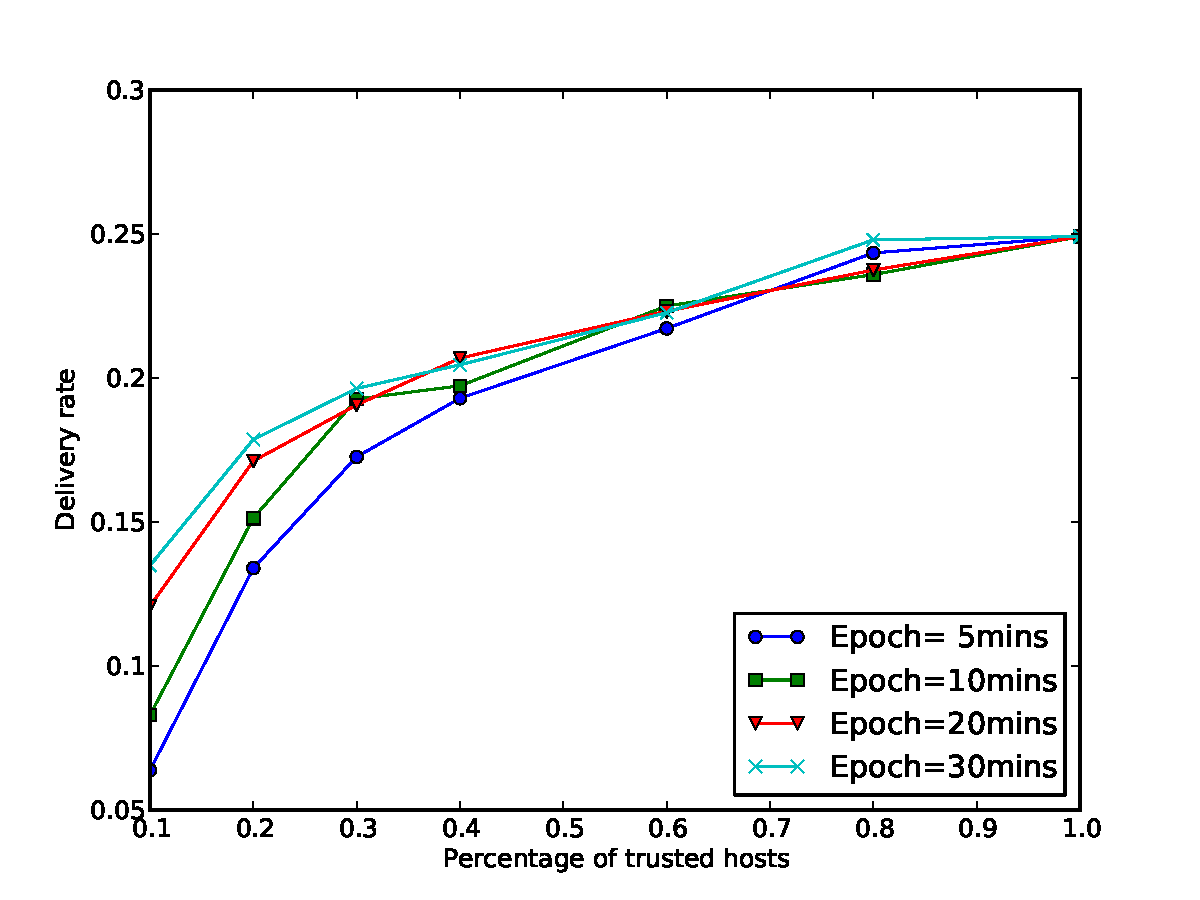
\includegraphics[width=0.49\columnwidth]{figures/epoch_1/delivery_rate.pdf}
\label{fig:delivery_rate_1}
}
\hfill
\subfloat[Delivery rate: Ephemeral ID valid for 3 epochs]{%
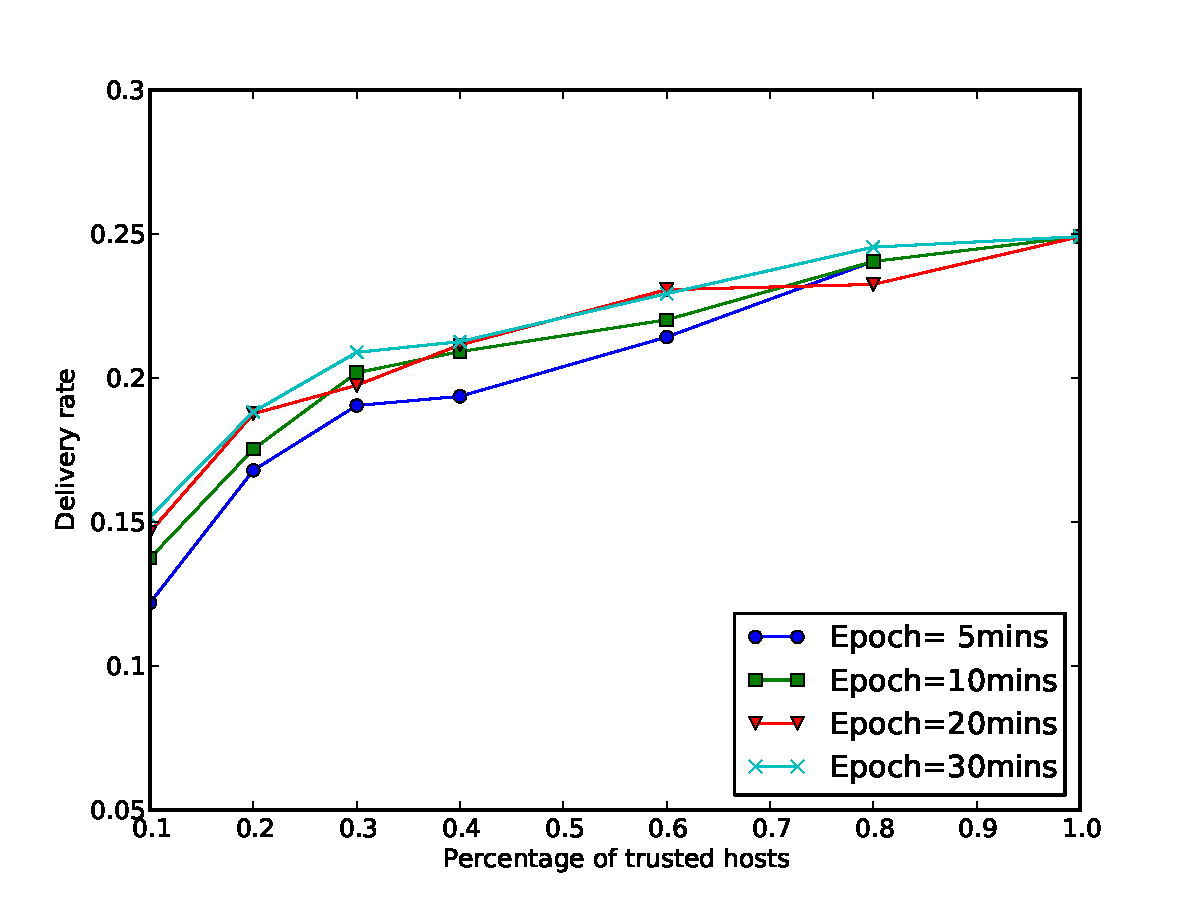
\includegraphics[width=0.49\columnwidth]{figures/epoch_3/delivery_rate.pdf}
\label{fig:delivery_rate_3}
}
\caption{{\bf Packet delivery rate.} 
Delivery rate with $100\%$ trusted nodes is exactly same to that of pure epidemic routing protocol (Delivery rate of 24.91\%). 
Delivery rate with 30 min epoch in Figure~\ref{fig:delivery_rate_1} and delivery rate with 10 min epoch in Figure~\ref{fig:delivery_rate_3} show almost similar result. 
}
\label{fig:delivery_rate}
\end{figure}




% delivery latency
\begin{figure}[h!]
\center
\subfloat[Delivery latency: Ephemeral ID valid for 1 epoch]{%
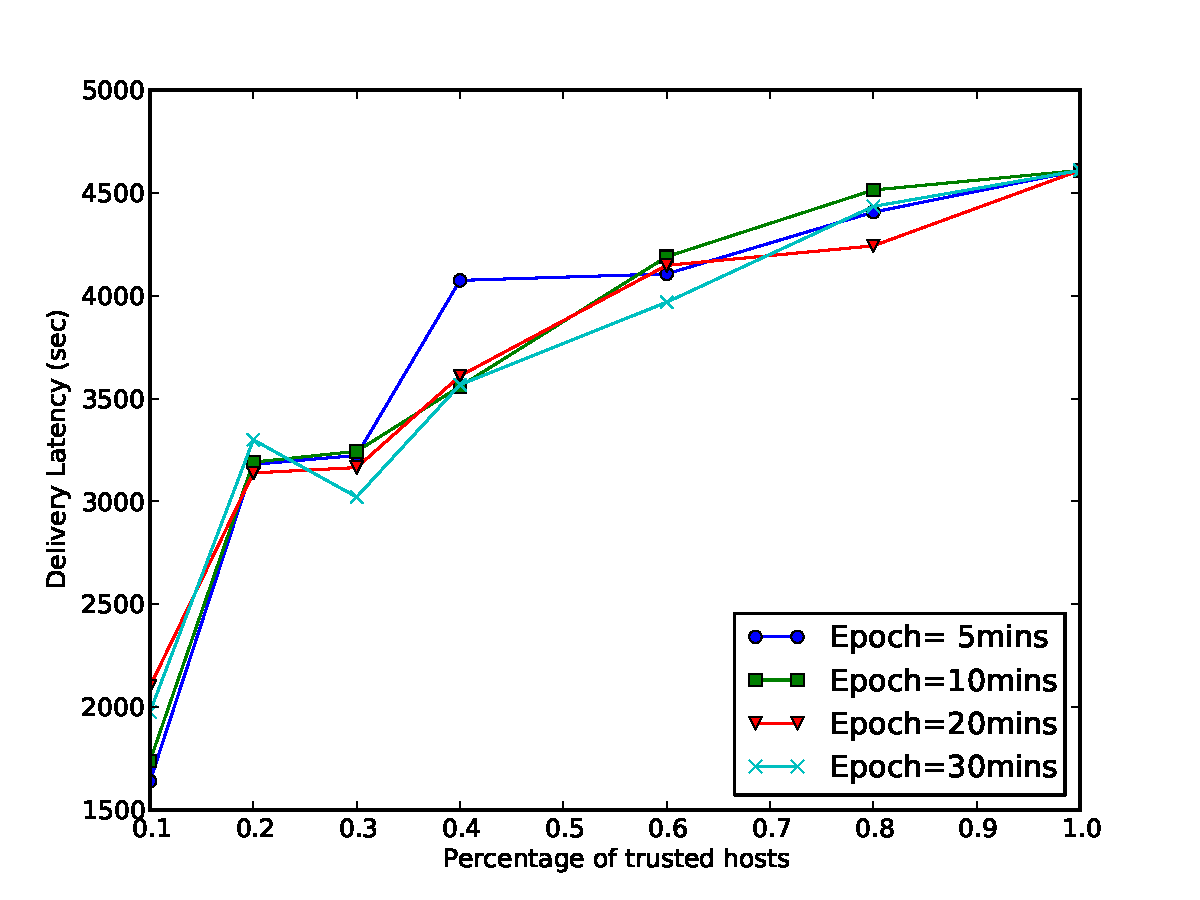
\includegraphics[width=0.49\columnwidth]{figures/epoch_1/delivery_latency.pdf}
\label{fig:delivery_latency_1}
}
\hfill
\subfloat[Delivery latency: Ephemeral ID valid for 3 epochs]{%
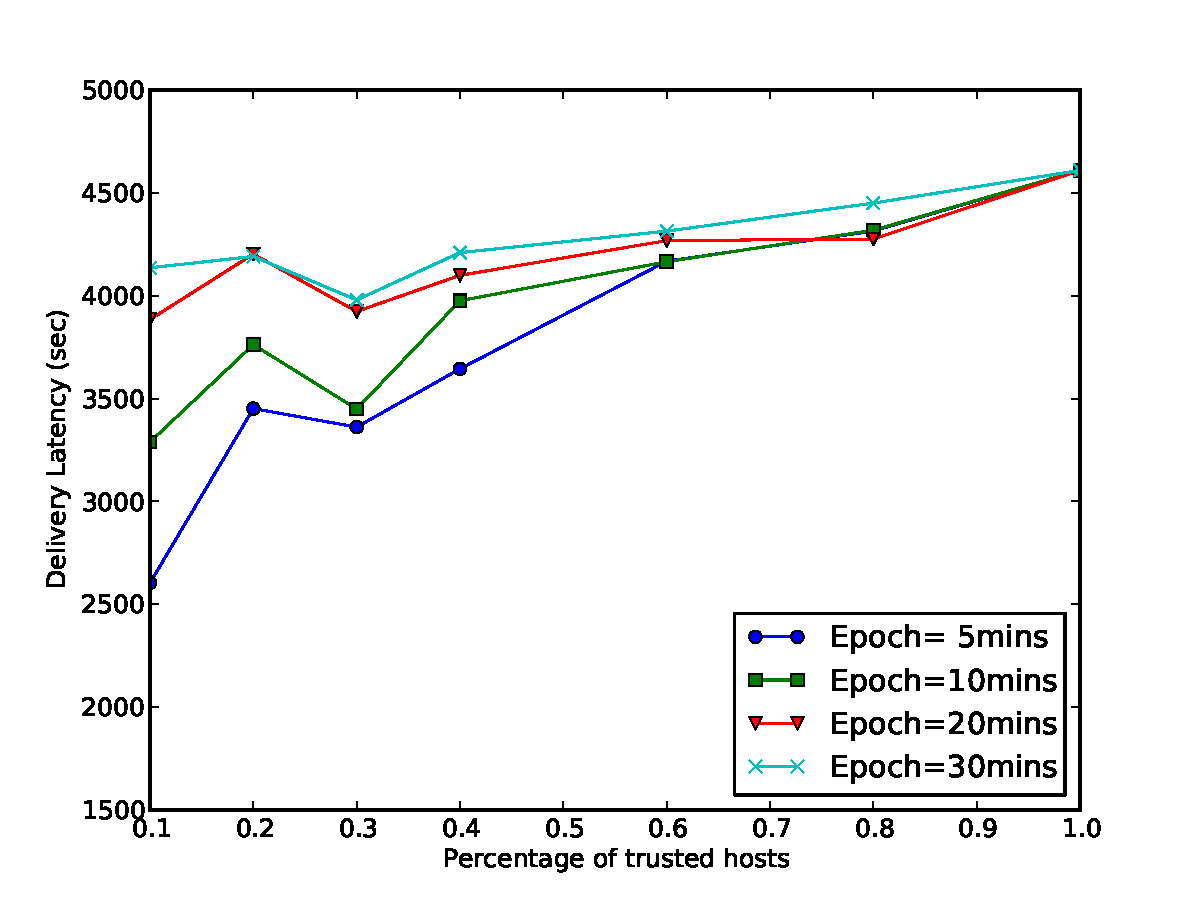
\includegraphics[width=0.49\columnwidth]{figures/epoch_3/delivery_latency.pdf}
\label{fig:delivery_latency_3}
}
\caption{{\bf Packet delivery latency.}
Packet delivery latency in Figure~\ref{fig:delivery_latency_3} is much higher than in Figure~\ref{fig:delivery_latency_1}, especially when the percentage of trusted nodes is low.
}
\label{fig:delivery_latency}
\end{figure}



% hop count
\begin{figure}[h!]
\center
\subfloat[Delivery hop count: Ephemeral ID valid for 1 epoch]{%
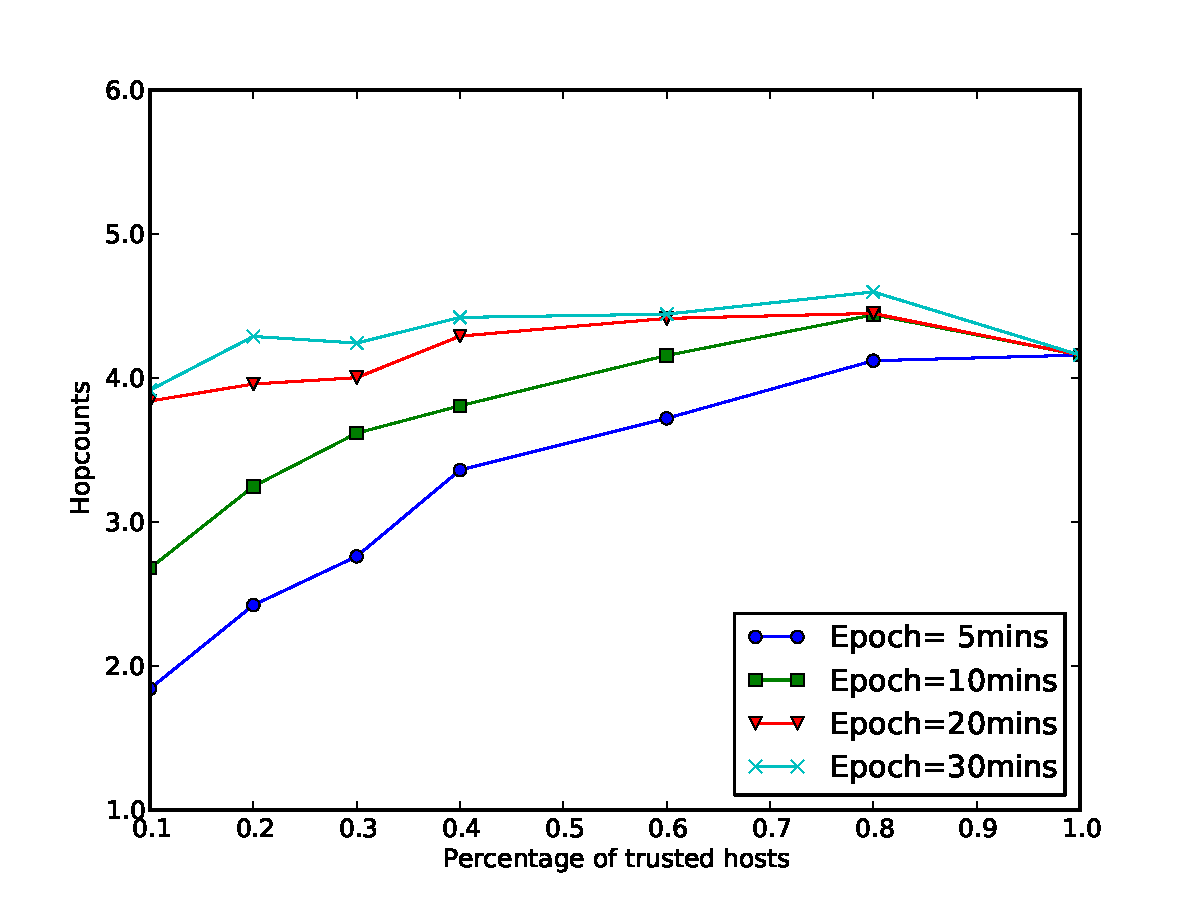
\includegraphics[width=0.49\columnwidth]{figures/epoch_1/hopcount.pdf}
\label{fig:delivery_hopcount_1}
}
\hfill
\subfloat[Delivery hop count: Ephemeral ID valid for 3 epochs]{%
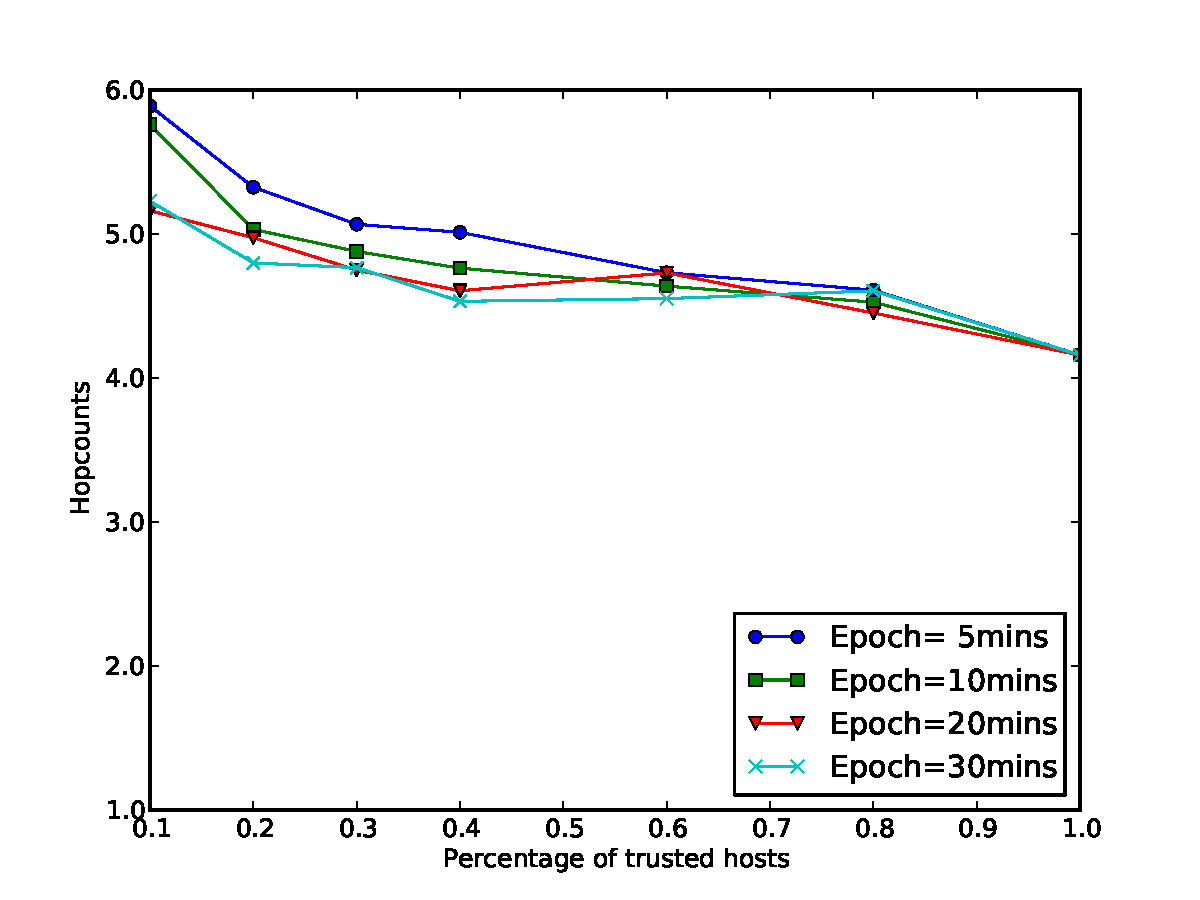
\includegraphics[width=0.49\columnwidth]{figures/epoch_3/hopcount.pdf}
\label{fig:delivery_hopcount_3}
}
\caption{{\bf Packet delivery hop count.}
Delivery hop count in Figure \ref{fig:delivery_hopcount_1} is generally lower than that of pure epidemic routing, since packets are dropped due to ephemeral ID expiry.  
Delivery hop count in Figure \ref{fig:delivery_hopcount_3} is generally higher than that of pure epidemic routing, especially when the percentage of trusted nodes is low due to inefficient routing using small number of trusted nodes.
}
\label{fig:delivery_hopcount}
\end{figure}




% overall packet relay count / delivered packet relay count 
\begin{figure}[h!]
\center
\subfloat[Relay count of overall packets. Ephemeral ID valid for 1 epoch.]{%
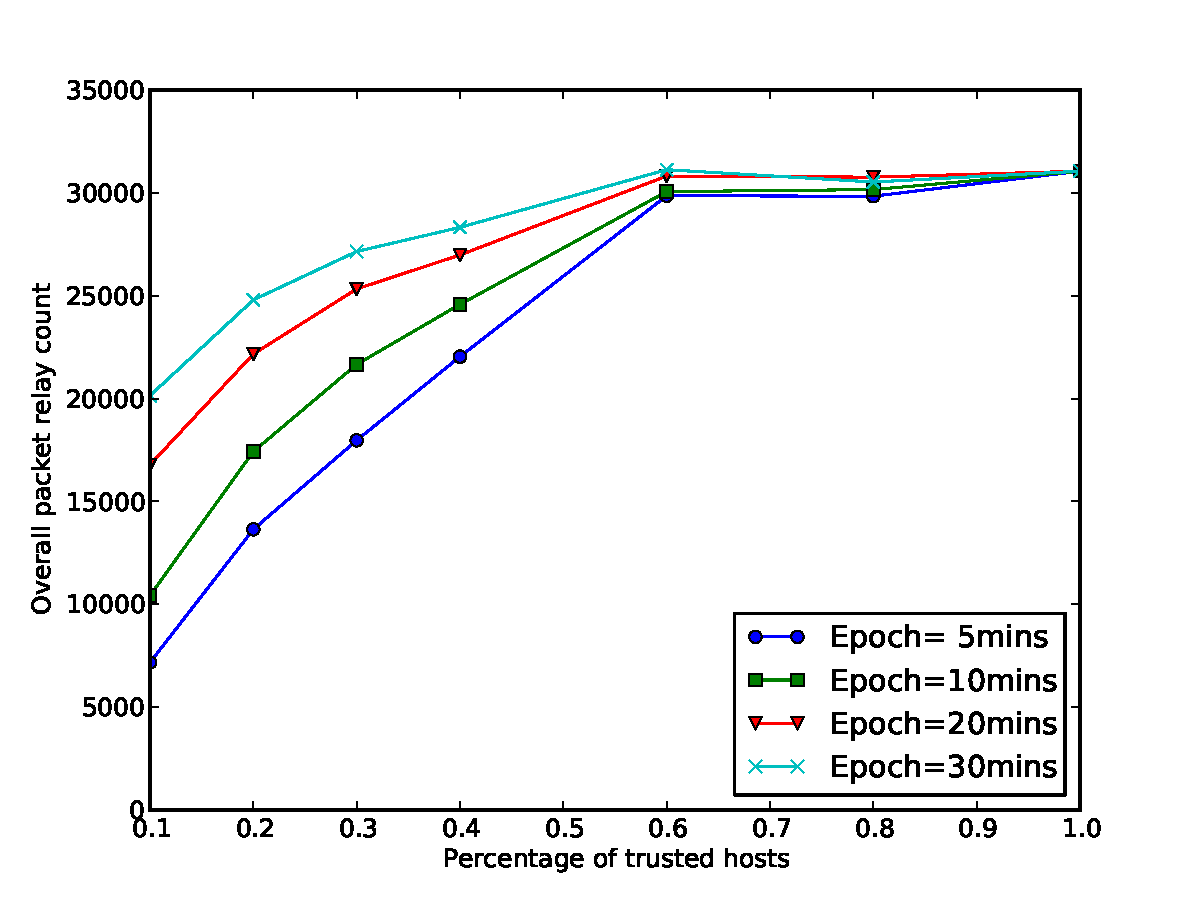
\includegraphics[width=0.49\columnwidth]{figures/epoch_1/relay_count.pdf}
\label{fig:relay_count_epoch_1}
}
\hfill
\subfloat[Relay count of overall packets. Ephemeral ID valid for 3 epochs.]{%
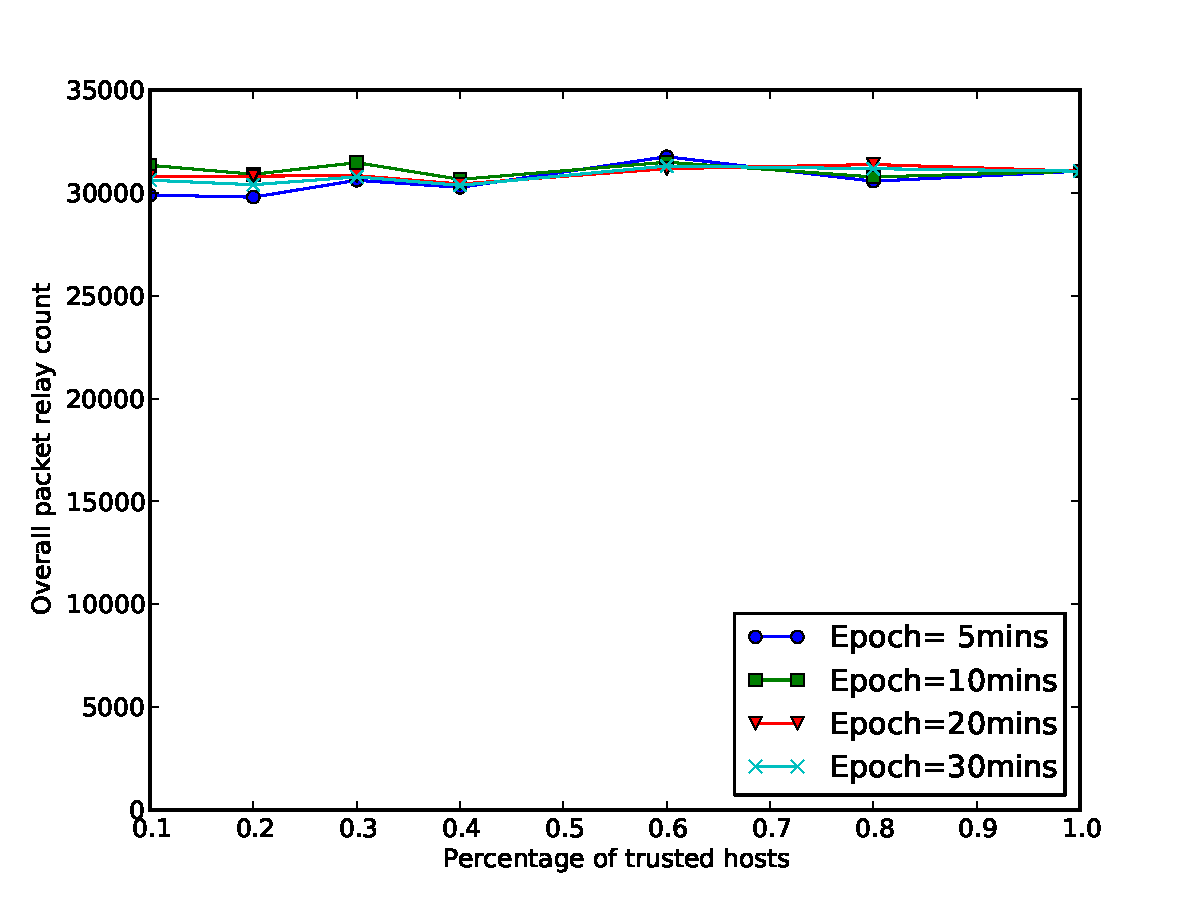
\includegraphics[width=0.49\columnwidth]{figures/epoch_3/relay_count.pdf}
\label{fig:relay_count_epoch_3}
}
\hfill
\subfloat[Relay count of delivered packets only. Ephemeral ID valid for 1 epoch.]{%
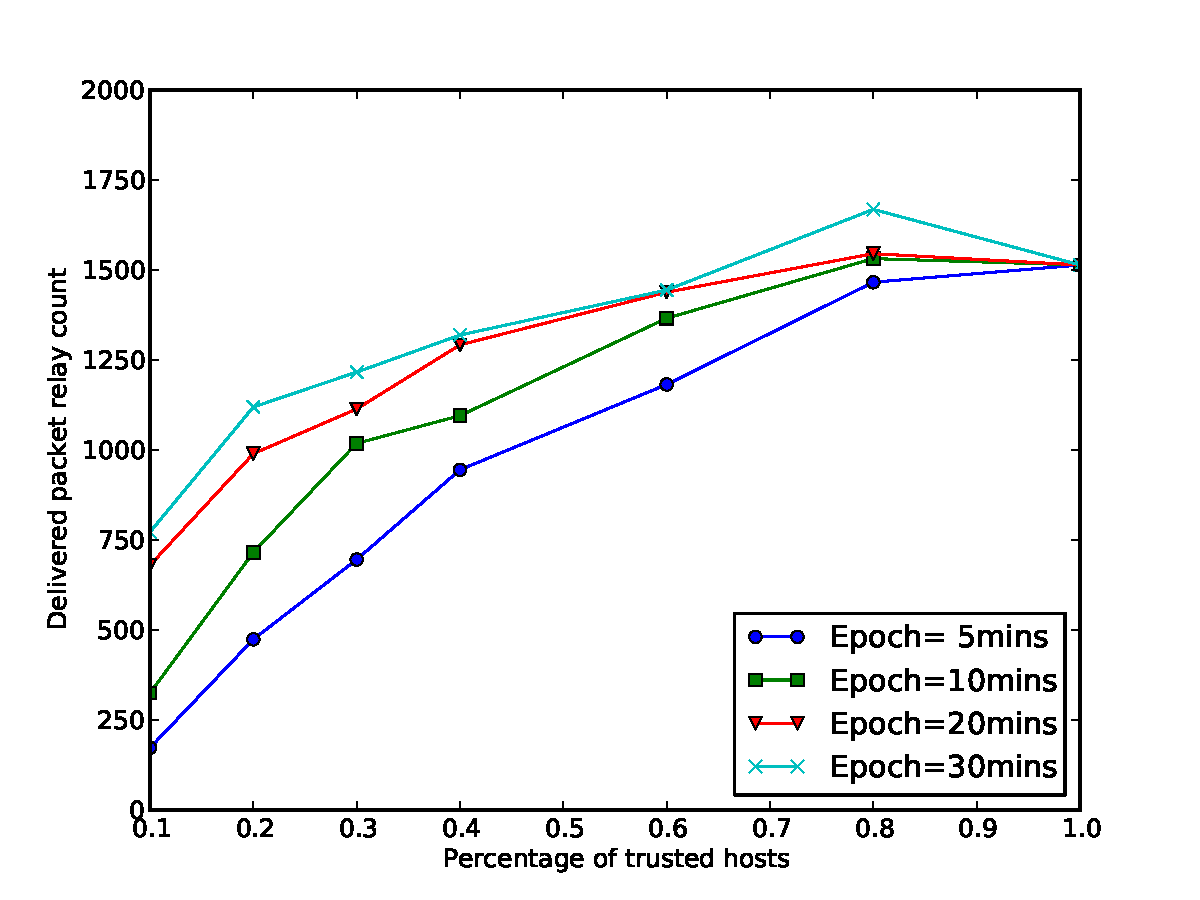
\includegraphics[width=0.49\columnwidth]{figures/epoch_1/relay_delivery_count.pdf}
\label{fig:relay_delivery_count_epoch_1}
}
\hfill
\subfloat[Relay count of delivered packets only. Ephemeral ID valid for 3 epochs.]{%
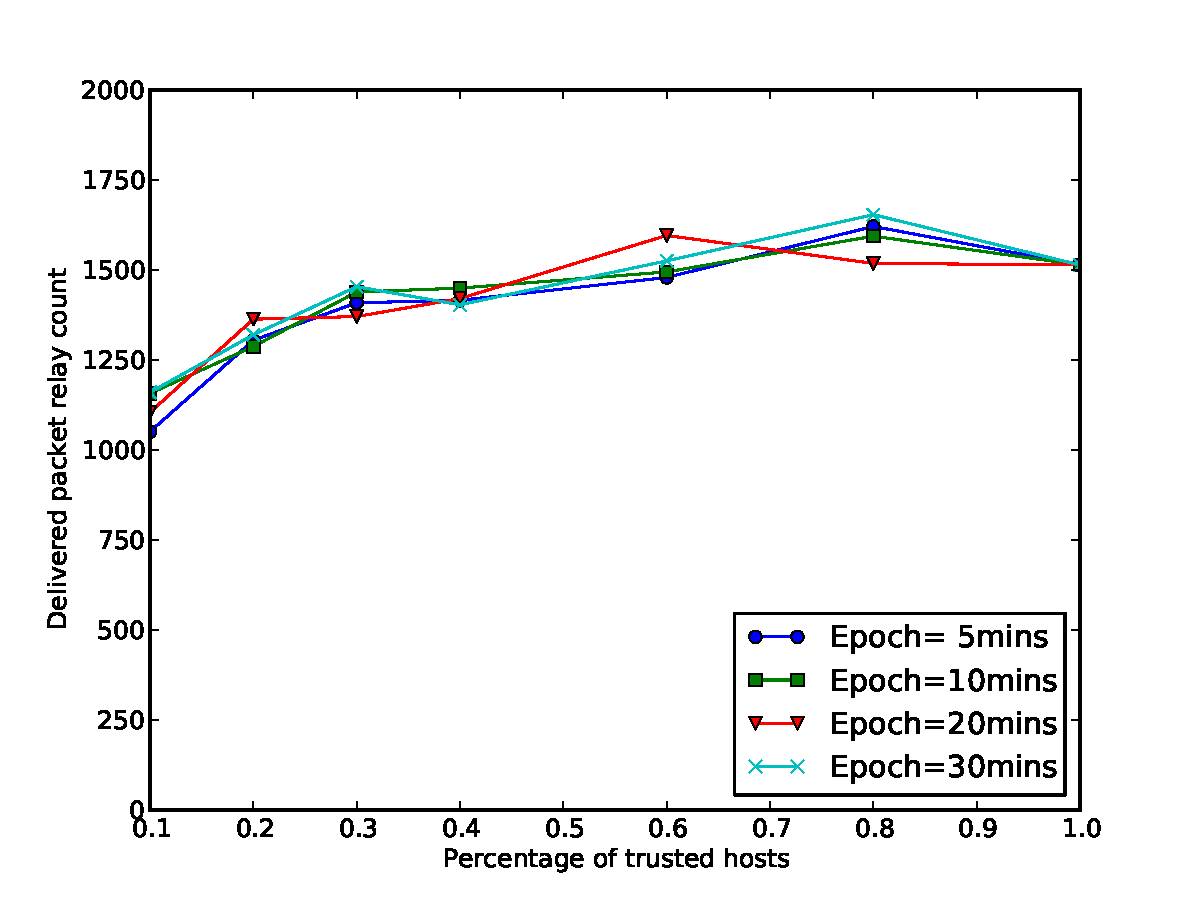
\includegraphics[width=0.49\columnwidth]{figures/epoch_3/relay_delivery_count.pdf}
\label{fig:relay_delivery_count_epoch_3}
}
\hfill

\caption{{\bf Packet relay count.}
In flood-based routing protocol, only about $5\%$ of packet relays are used for actual packet deliveries. 
When ephemeral ID valid for 3 epochs is used (Figures~\ref{fig:relay_count_epoch_3} and \ref{fig:relay_delivery_count_epoch_3}), 
the number of packet relays (both overall packet relays and delivered packet relays) are significantly increased, 
especially when the percentage of trusted nodes is less than $60\%$.}
\label{fig:relay_count}
\end{figure}







% packet relay classification over varying eppoch
\begin{figure}[h!]
\center
\subfloat[Overall packet relay classification. Ephemeral ID valid for 1 epoch]{%
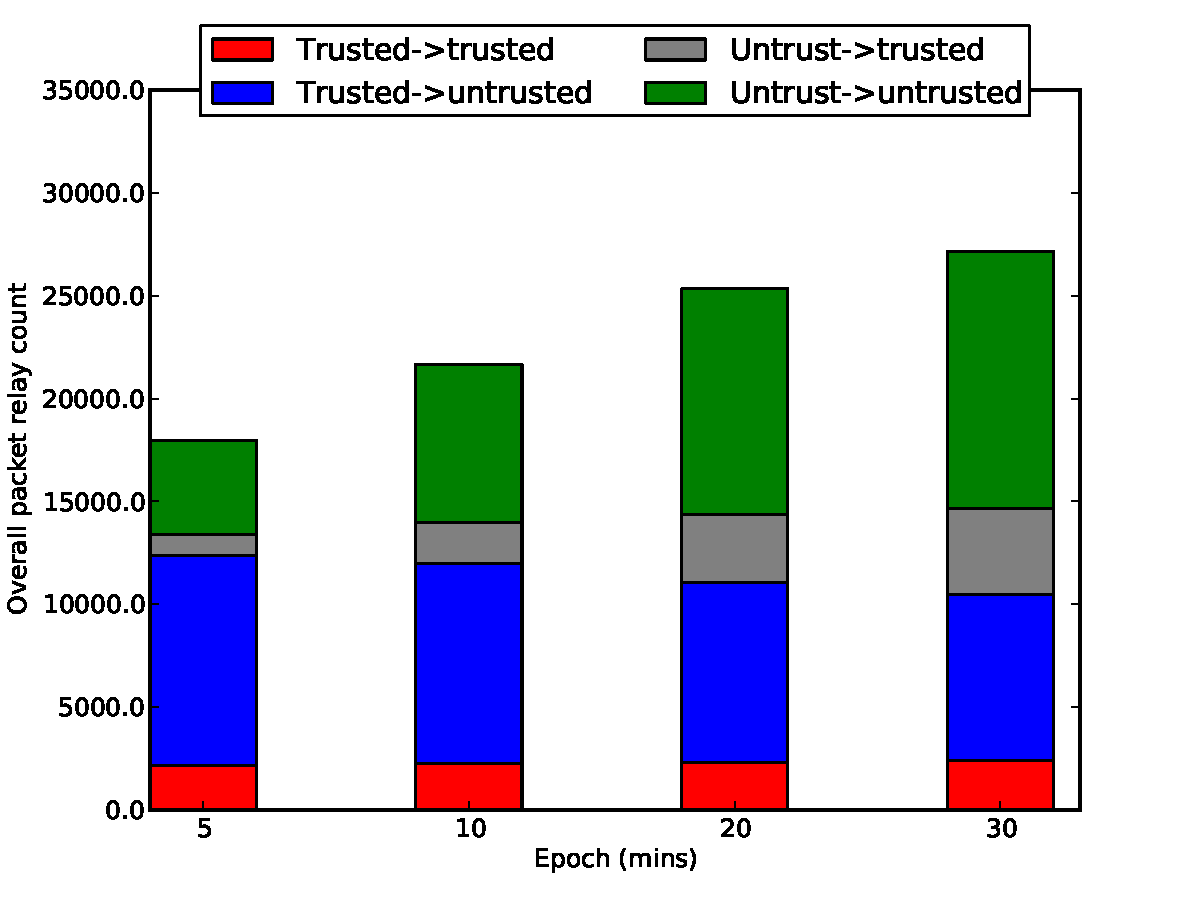
\includegraphics[width=0.49\columnwidth]{figures/epoch_1/relay_classification_over_epoch.pdf}
\label{fig:overall_relay_classification_epoch_1}
}
\hfill
\subfloat[Overall packet relay classification. Ephemeral ID valid for 3 epochs]{%
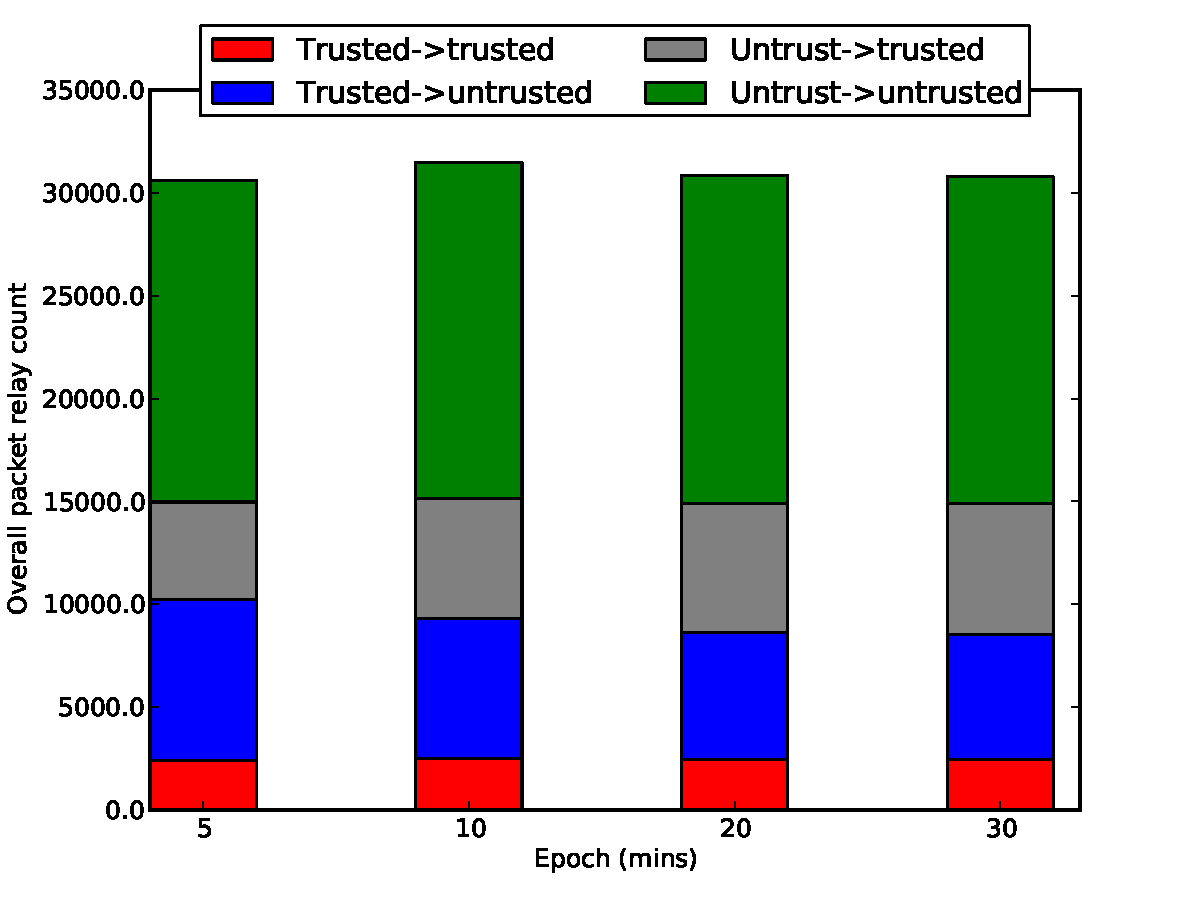
\includegraphics[width=0.49\columnwidth]{figures/epoch_3/relay_classification_over_epoch.pdf}
\label{fig:overall_relay_classification_epoch_3}
}
\hfill
\subfloat[Delivered packet relay classification. Ephemeral ID valid for 1 epoch]{%
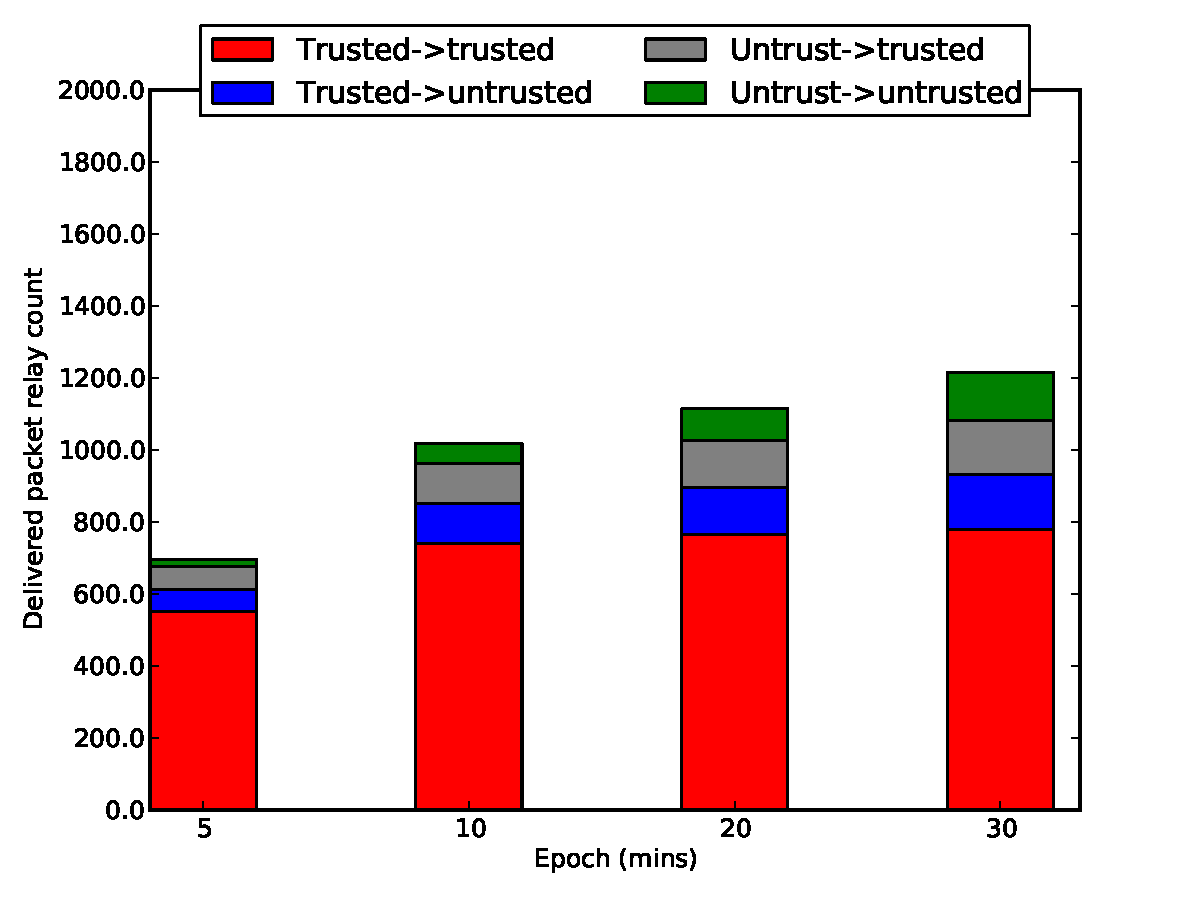
\includegraphics[width=0.49\columnwidth]{figures/epoch_1/relay_delivery_classification_over_epoch.pdf}
\label{fig:delivered_relay_classification_epoch_1}
}
\hfill
\subfloat[Delivered packet relay classification. Ephemeral ID valid for 3 epochs]{%
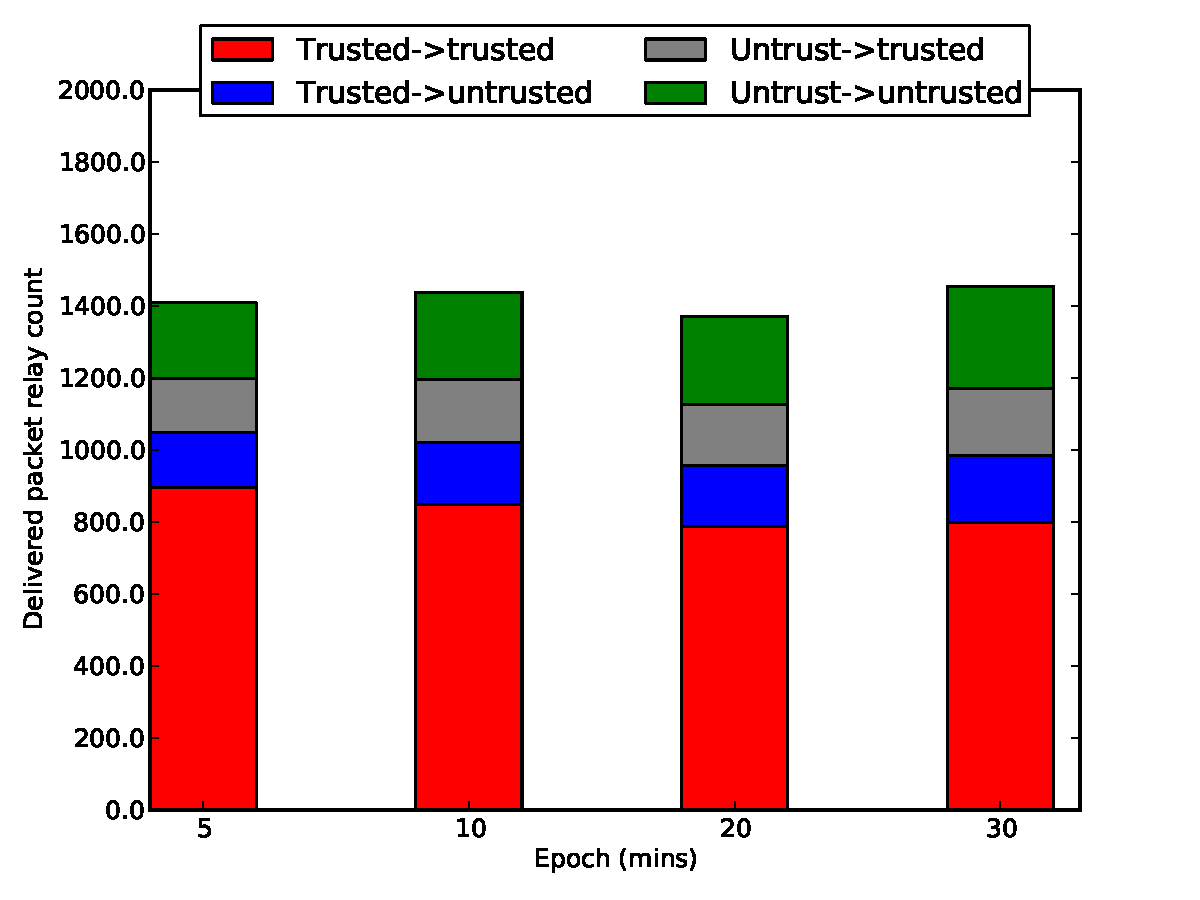
\includegraphics[width=0.49\columnwidth]{figures/epoch_3/relay_delivery_classification_over_epoch.pdf}
\label{fig:delivered_relay_classification_epoch_3}
}

\caption{{\bf Packet relay classification over varying epoch. Percentage of trusted nodes is $30\%$.}
Relays between two trusted nodes account for $10\%$ to $20\%$ in overall packet relay classification,
but relays between two trusted nodes account for more than $60\%$ in delivered packet relay classification.
In addition, relays between two untrusted nodes account for $25\%$ to $50\%$ in overall packet relay classification, 
but it accounts only for less than $15\%$ in delivered packet relay classification. 
}
\label{fig:relay_classification_epoch}
\end{figure}




% packet relay classification over varying percentage of trusted nodes
\begin{figure}[h!]
\center
\subfloat[Overall packet relay classification. Ephemeral ID valid for 1 epoch.]{%
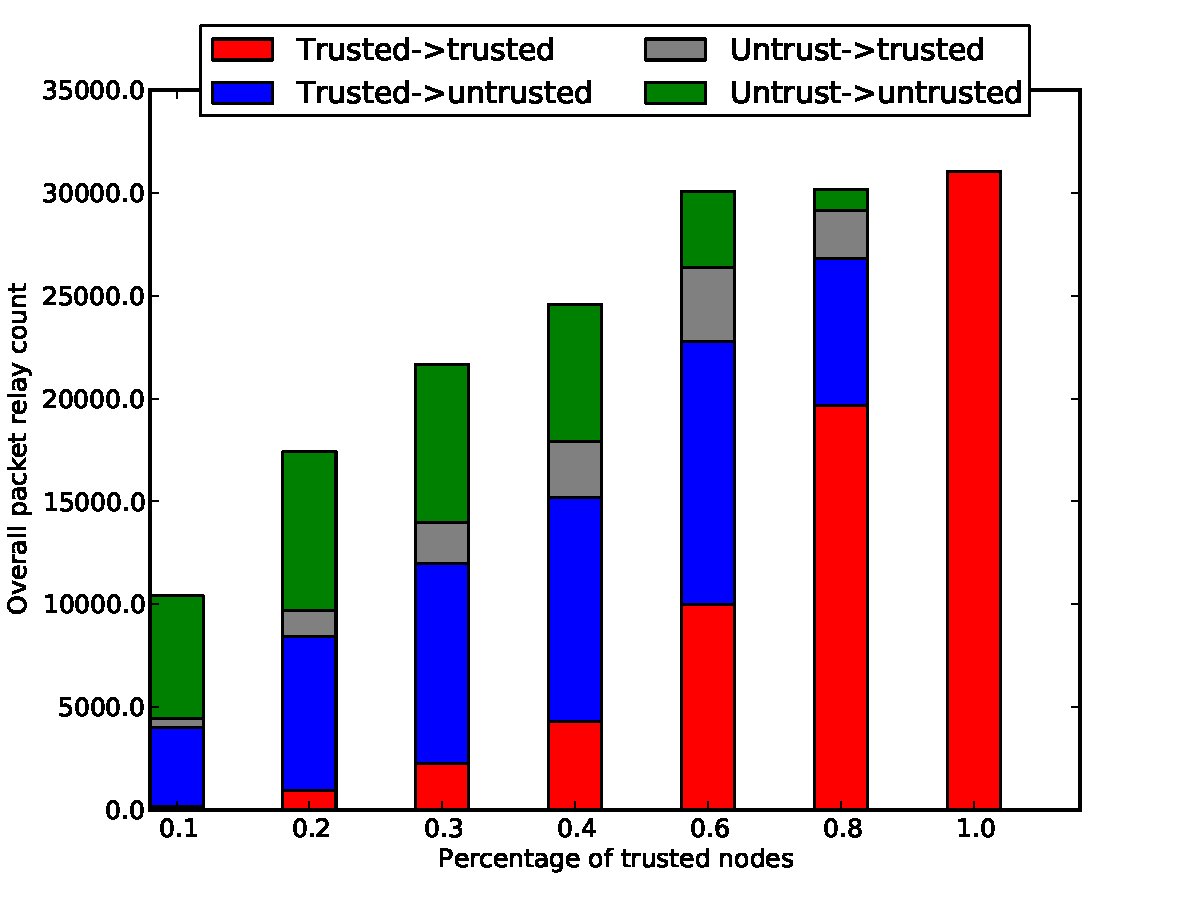
\includegraphics[width=0.49\columnwidth]{figures/epoch_1/relay_classification_over_percentage.pdf}
\label{fig:relay_classification_percentage_1}
}
\hfill
\subfloat[Overall packet relay classification. Ephemeral ID valid for 3 epochs.]{%
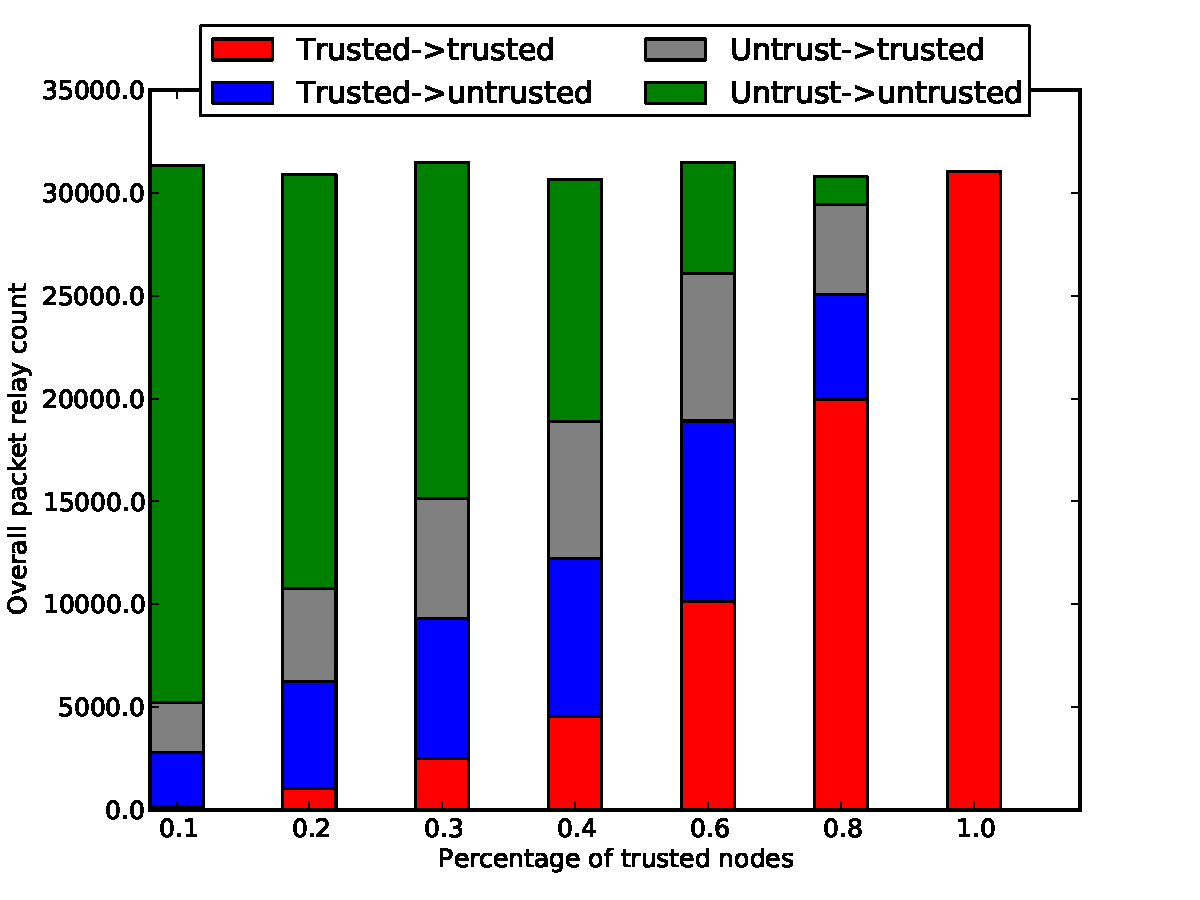
\includegraphics[width=0.49\columnwidth]{figures/epoch_3/relay_classification_over_percentage.pdf}
\label{fig:relay_classification_percentage_3}
}

\hfill
\subfloat[Delivered packet relay classification. Ephemeral ID valid for 1 epoch.]{%
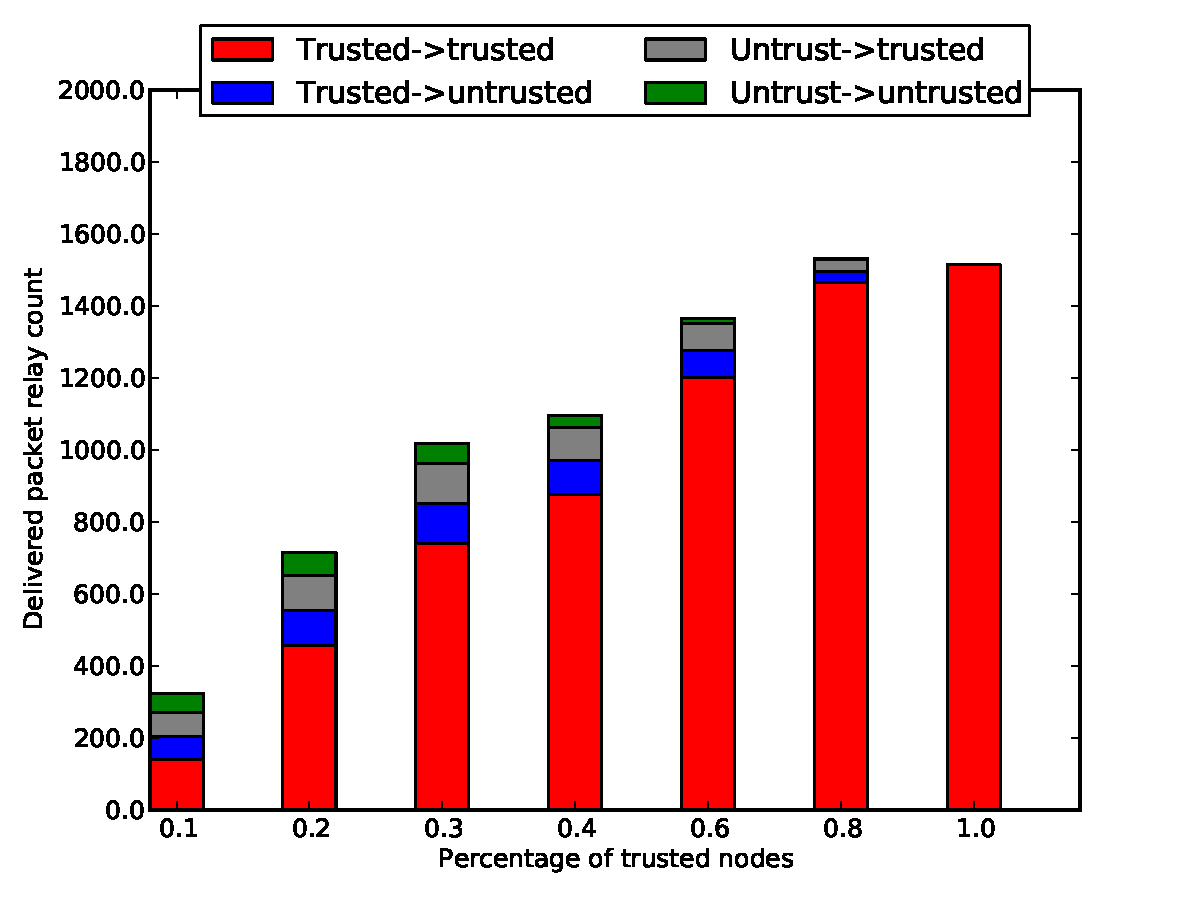
\includegraphics[width=0.49\columnwidth]{figures/epoch_1/relay_delivery_classification_over_percentage.pdf}
\label{fig:delivered_relay_classification_percentage_1}
}
\hfill
\subfloat[Delivered packet relay classification. Ephemeral ID valid for 3 epochs.]{%{%
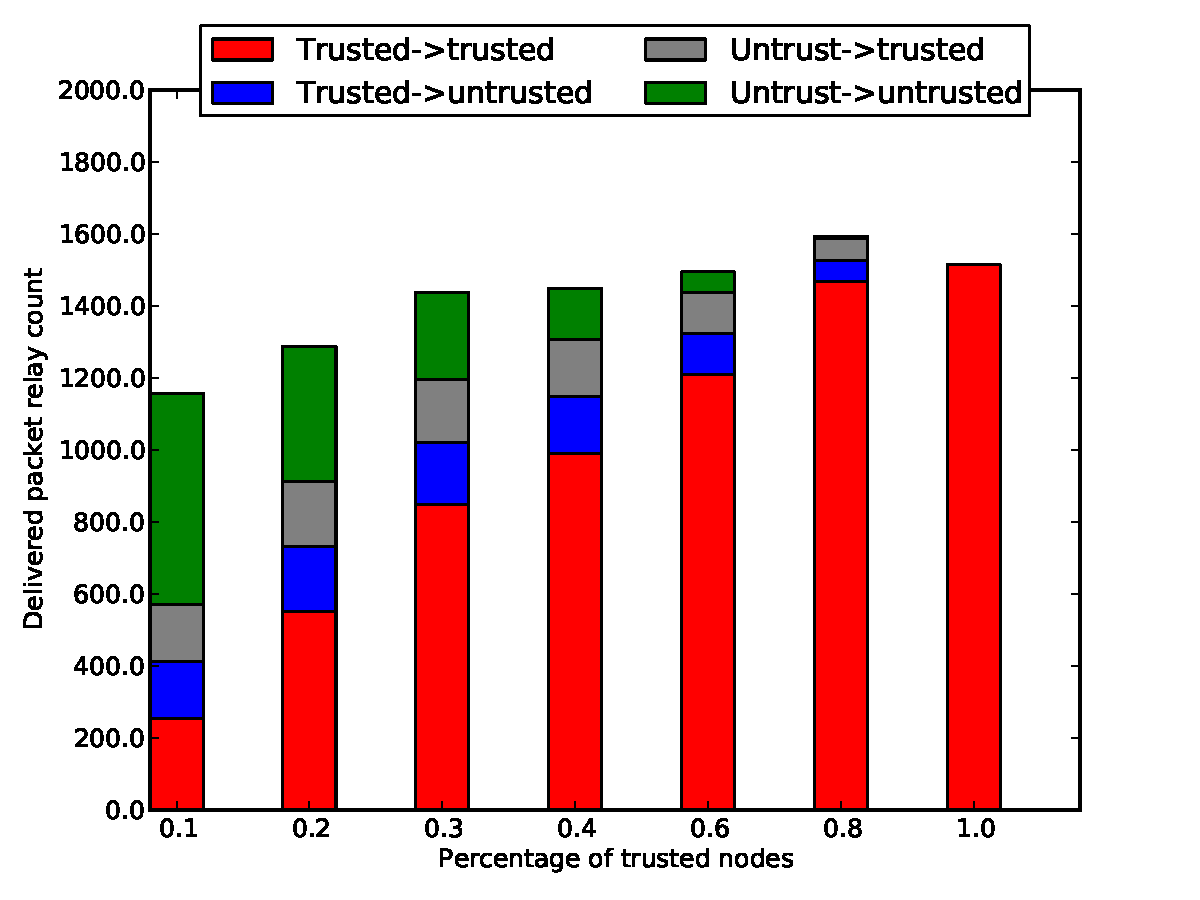
\includegraphics[width=0.49\columnwidth]{figures/epoch_3/relay_delivery_classification_over_percentage.pdf}
\label{fig:delivered_relay_classification_percentage_3}
}

\caption{{\bf Packet relay classification over varying percentage of trusted nodes. Epoch is $10$ mins.}
As in Figure~\ref{fig:relay_classification_epoch}, relays between two untrusted nodes account for relatively small part while relays between two trusted nodes account for the largest part (in most cases) in delivered packet relay classification. 
}
\label{fig:relay_classification_percentage}
\end{figure}




% packet drop classification
\begin{figure}[h!]
\center
\subfloat[Packet drops over varied epoch. Percentage of trusted nodes = 0.3. Ephemeral ID valid for 1 epoch.]{%
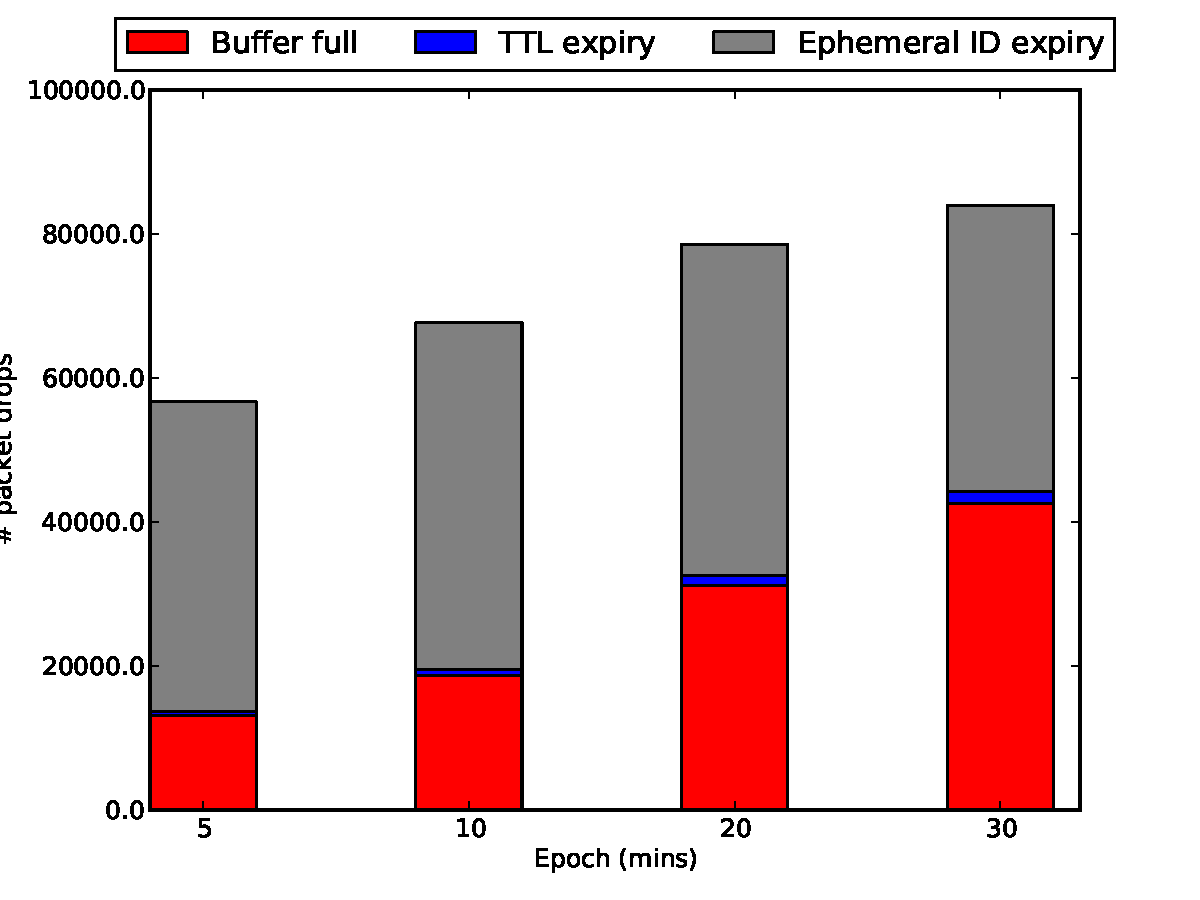
\includegraphics[width=0.49\columnwidth]{figures/epoch_1/drop_classification_over_epoch.pdf}
\label{fig:drop_classification_epoch_1}
}
\hfill
\subfloat[Packet drops over varied epoch. Percentage of trusted nodes = 0.3. Ephemeral ID valid for 3 epochs.]{%
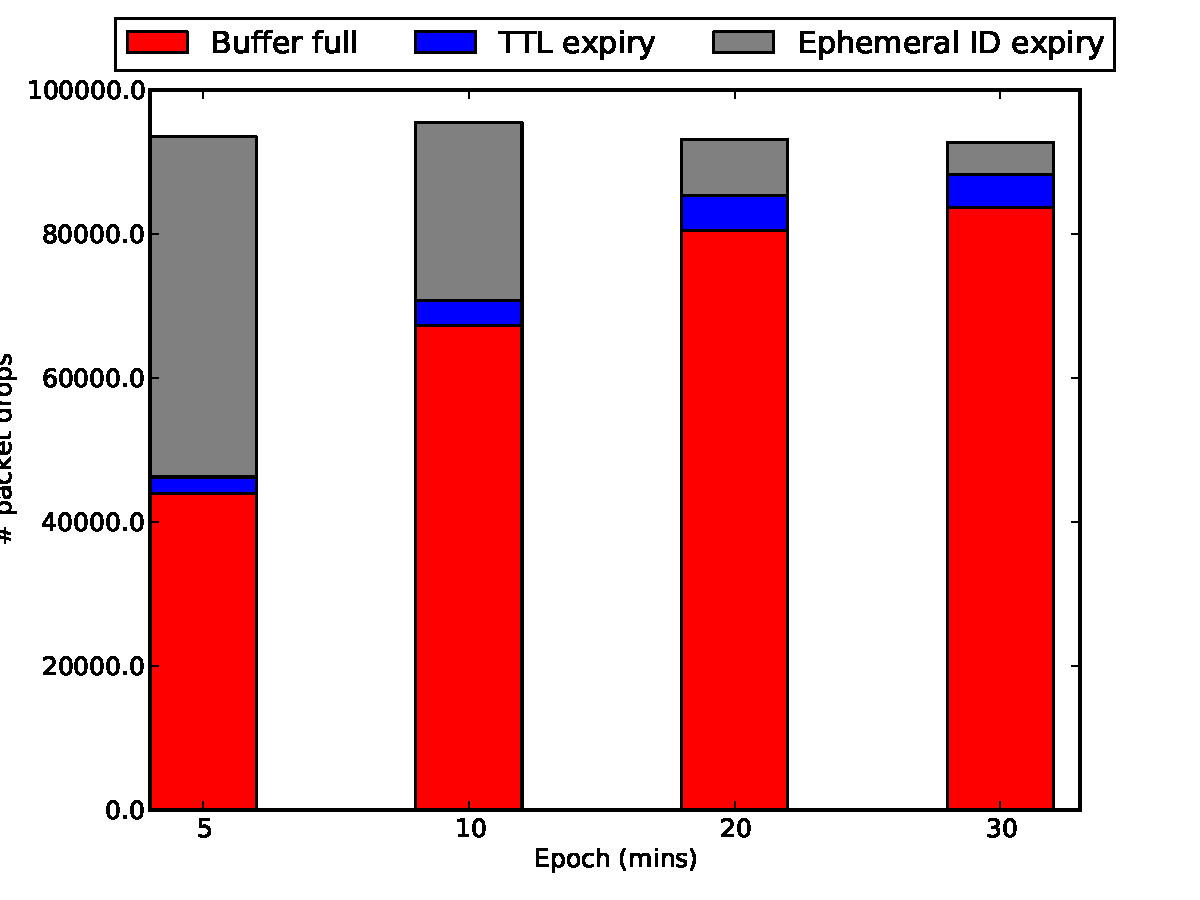
\includegraphics[width=0.49\columnwidth]{figures/epoch_3/drop_classification_over_epoch.pdf}
\label{fig:drop_classification_epoch_3}
}
\hfill
\subfloat[Packet drops over varied percentage of trusted nodes. Epoch = 10 mins. Ephemeral ID valid for 1 epoch.]{%
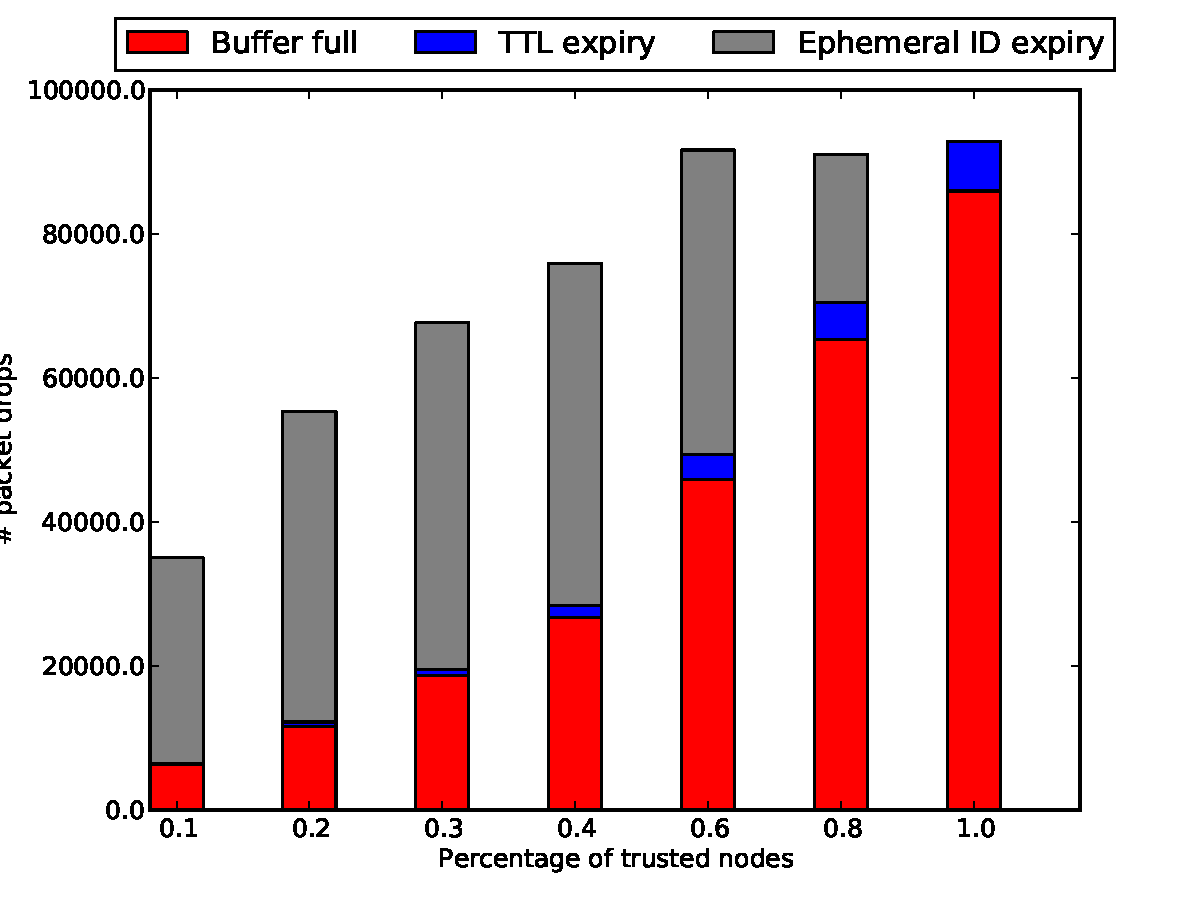
\includegraphics[width=0.49\columnwidth]{figures/epoch_1/drop_classification_over_percentage.pdf}
\label{fig:drop_classification_percentage_1}
}
\subfloat[Packet drops over varied percentage of trusted nodes. Epoch = 10 mins. Ephemeral ID valid for 3 epochs.]{%
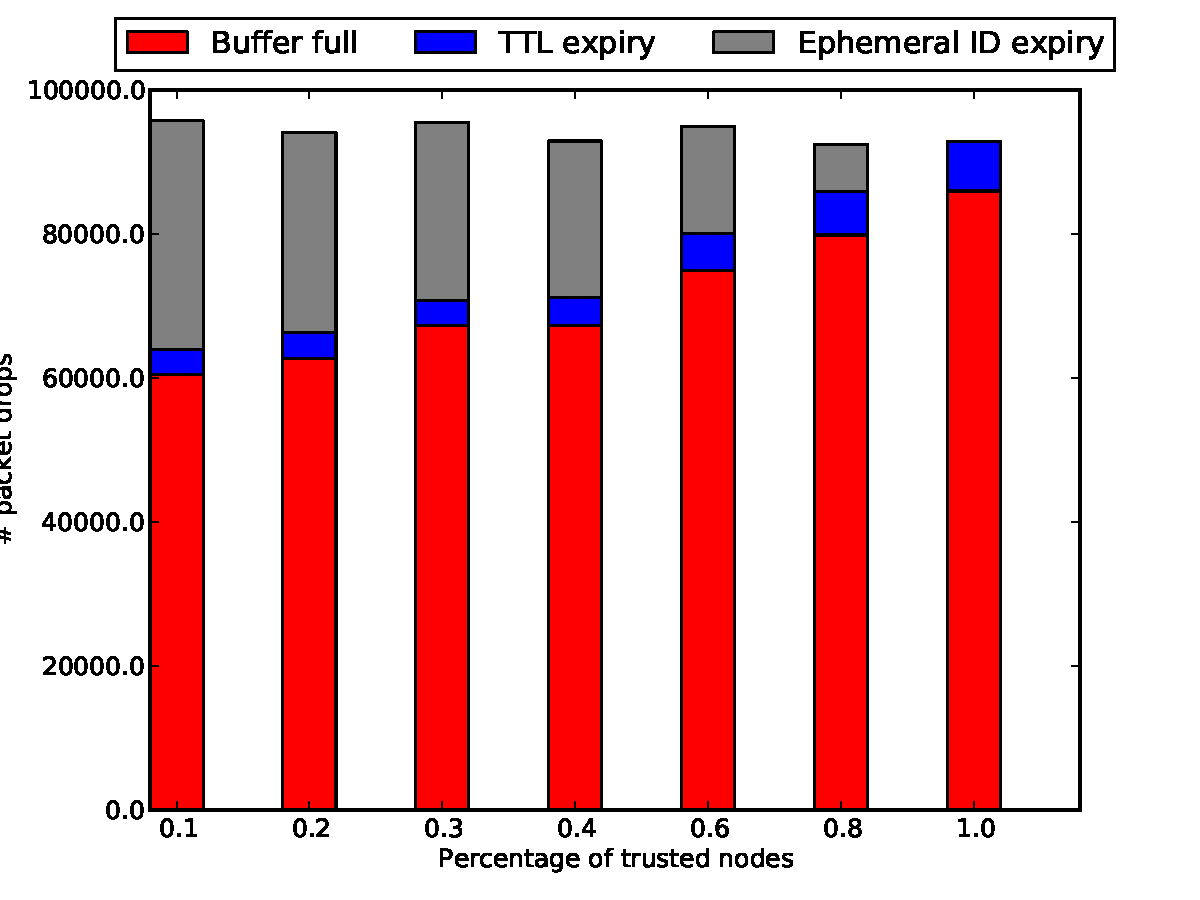
\includegraphics[width=0.49\columnwidth]{figures/epoch_3/drop_classification_over_percentage.pdf}
\label{fig:drop_classification_percentage_3}
}
\caption{{\bf Packet drop classification.}
With ephemeral ID valid for 3 epochs (Figures~\ref{fig:drop_classification_epoch_3} and \ref{fig:drop_classification_percentage_3}),  
the total number of packet drops is significantly increased compared to when ephemeral ID valid for 1 epoch is used (Figures~\ref{fig:drop_classification_epoch_1} and \ref{fig:drop_classification_percentage_1}).
However, most packet drops are due to buffer overflow, and packet drops due to ephemeral ID expiry is significantly decreased. 
}
\label{fig:drop_classification}
\end{figure}






% packet delivery count with untrusted nodes
\begin{figure}[t!]
\center
\subfloat[Packet deliveries with untrusted nodes: Ephemeral ID valid for 1 epoch.]{%
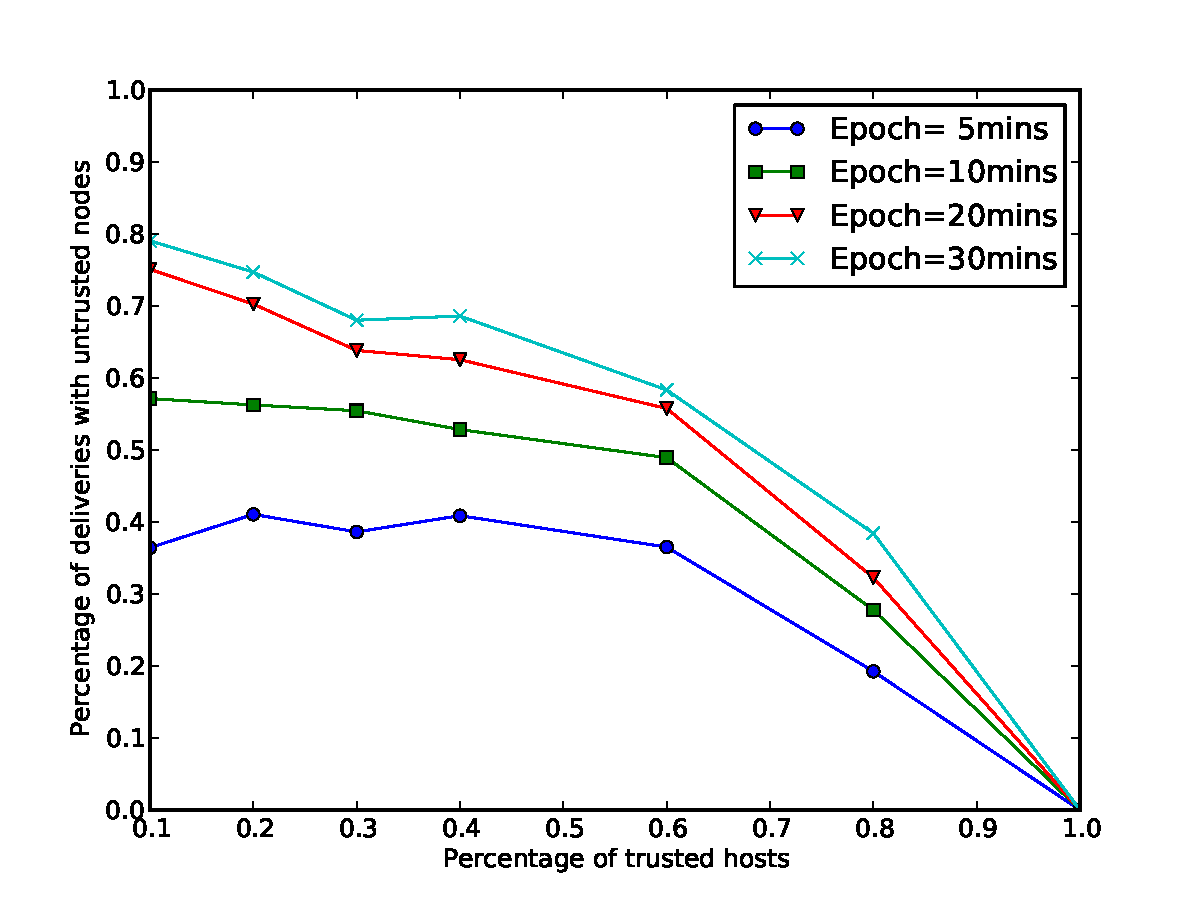
\includegraphics[width=0.49\columnwidth]{figures/epoch_1/delivery_with_ut.pdf}
\label{fig:delivery_ut_1}
}
\hfill
\subfloat[Packet deliveries with untrusted nodes: Ephemeral ID valid for 3 epochs.]{%
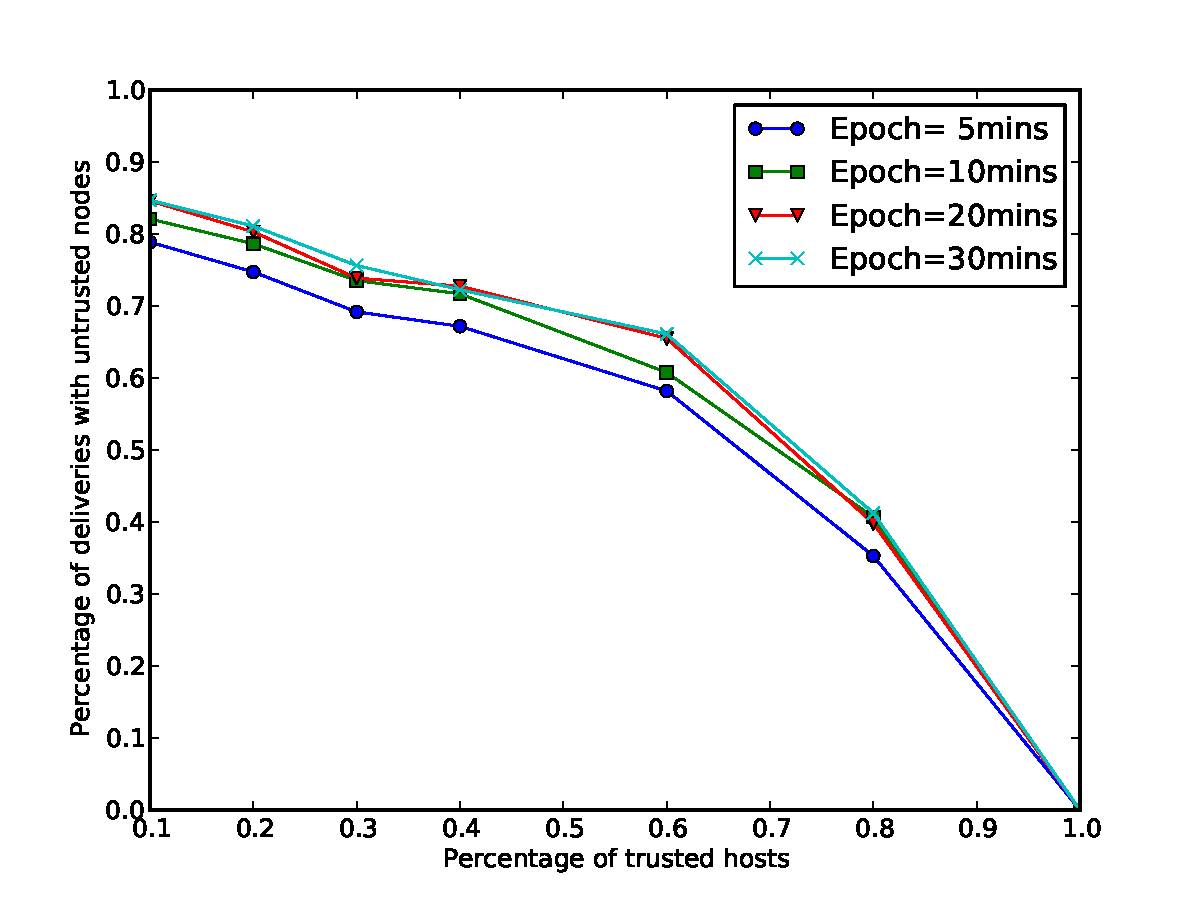
\includegraphics[width=0.49\columnwidth]{figures/epoch_3/delivery_with_ut.pdf}
\label{fig:delivery_ut_3}
}
\caption{{\bf Packet deliveries with untrusted nodes.}
The number Packet deliveries including at least 1 untrusted node is significantly increased with the use of ephemeral ID valid for 3 epochs. 
}
\label{fig:delivery_count}
\end{figure}




% average relay count per message
\begin{comment}
\begin{figure}[h!]
\center
\subfloat[Average relay count per message. Ephemeral ID valid for 1 epoch]{%
\includegraphics[width=0.49\columnwidth]{figures/epoch_1/relay_per_message.pdf}
\label{fig:relay_per_message_1}
}
\hfill
\subfloat[Average relay count per message. Ephemeral ID valid for 3 epochs]{%
\includegraphics[width=0.49\columnwidth]{figures/epoch_3/relay_per_message.pdf}
\label{fig:relay_per_message_3}
}
\caption{{\bf Average relay counts per message.}
With ephemeral ID valid for 1 epoch, packets are not relayed enough times since the packets are dropped mainly due to ephemeral ID expiry, especially when the percentage of trusted node is low (Figure~\ref{fig:relay_per_message_1}). 
By using ephemeral ID valid for 3 epochs, the average relay count per message stays almost same regardless of the percentage of trusted nodes.
}
\label{fig:relay_per_message}
\end{figure}
\end{comment}



\end{document}







